\section{Resultados e discussão dos resultados}

\color{blue}\textit{Acredito que deva haver um modo bem melhor para organizar tudo isso, eu posso reunir gráficos em blocos? Assim como foi feito para os mapas de registros e espécies (até porque há 14 páginas só de imagens).}\color{black}

\subsection{Análise Univariada}

\begin{figure}[h!]
\centering
{\scriptsize Tabela 1: Número de municípios amostrados, registros e espécies nos bancos de dados: WAV = Wikiaves, SLI = SpeciesLink, WAV2 = WAV com municípios redundantes em SLI.}
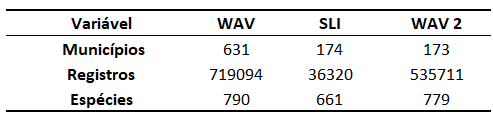
\includegraphics{Tabelas/1.png}
\label{t01}
\end{figure}

\begin{itemize}
    \item Registros por Município

\begin{figure}[h!]
\centering
{\scriptsize Tabela 2: Estatísticas de tendência central e dispersão para o número de registros por município em cada banco de dados: WAV = Wikiaves, SLI = SpeciesLink, WAV2 = WAV com municípios redundantes em SLI. Valores de média (m) e desvio-padrão (dp) em Log10 foram retrotransformados (Retro). min-max = valores extremos, q1-q3 = quartis.}
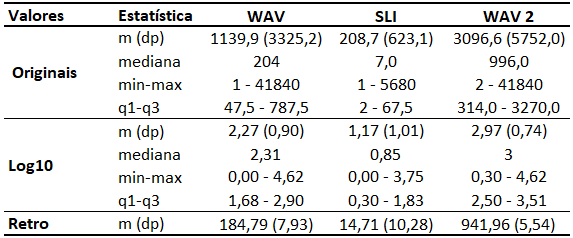
\includegraphics[height = 4cm]{Tabelas/2.png}
\label{t02}
\end{figure}

\begin{figure}[h!]
\centering
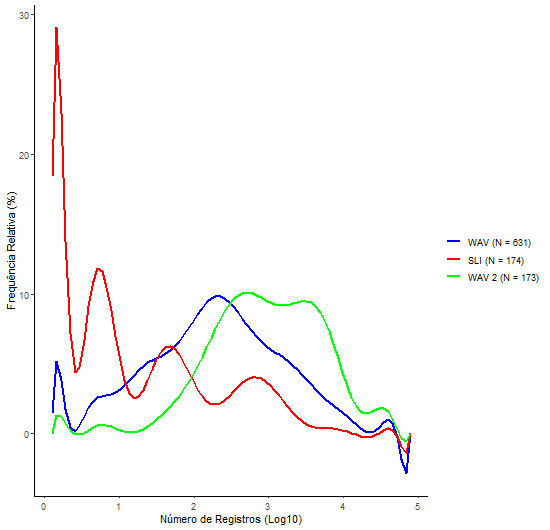
\includegraphics[height = 6cm]{Imagens/113.png}
\\{\scriptsize Figura 1: Distribuição de municípios em classes segundo o número de registros (Log10), em cada banco de dados: WAV = Wikiaves, SLI = SpeciesLink, WAV2 = WAV com municípios redundantes em SLI. n = número de municípios.  }
\label{fig01}
\end{figure}



\item Espécies por Município

\begin{figure}[h!]
\centering
{\scriptsize Tabela 3: Estatísticas de tendência central e dispersão para o número de espécies por município em cada banco de dados: WAV = Wikiaves, SLI = SpeciesLink, WAV2 = WAV com municípios redundantes em SLI. Valores de média (m) e desvio-padrão (dp) em Log10 foram retrotransformados (Retro). min-max = valores extremos, q1-q3 = quartis.}
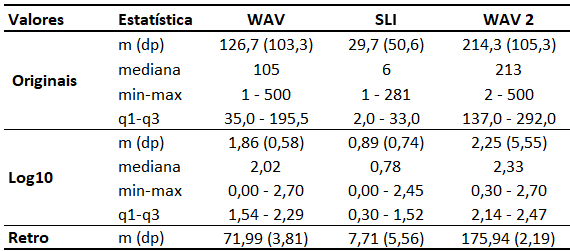
\includegraphics[height = 4cm]{Tabelas/3.png}
\label{t03}
\end{figure}


\begin{figure}[h!]
\centering
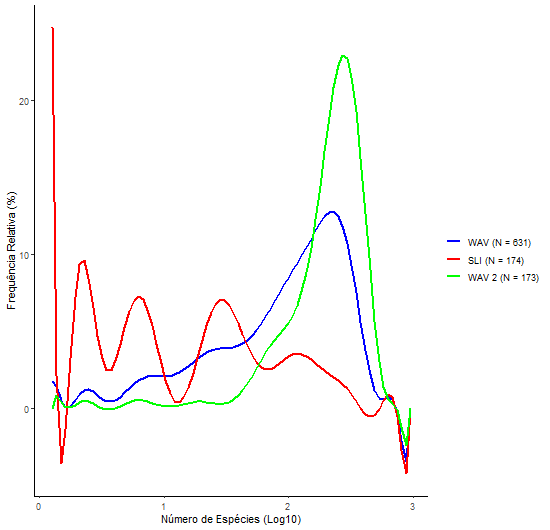
\includegraphics[height = 6cm]{Imagens/123.png}
\\{\scriptsize Figura 2: Distribuição de municípios em classes segundo o número de espécies (Log10), em cada banco de dados: WAV = Wikiaves, SLI = SpeciesLink, WAV2 = WAV com municípios redundantes em SLI. n = número de municípios. }
\label{fig02}
\end{figure}

\newpage

\item Registros por Espécie

\begin{figure}[h!]
\centering
{\scriptsize Tabela 4: Estatísticas de tendência central e dispersão para o número de registros por espécie em cada banco de dados: WAV = Wikiaves, SLI = SpeciesLink, WAV2 = WAV com municípios redundantes em SLI. Valores de média (m) e desvio-padrão (dp) em Log10 foram retrotransformados (Retro). min-max = valores extremos, q1-q3 = quartis.}
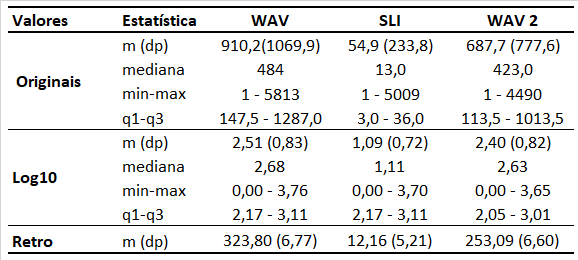
\includegraphics[height = 4cm]{Tabelas/4.png}
\label{t04}
\end{figure}

\begin{figure}[h!]
\centering
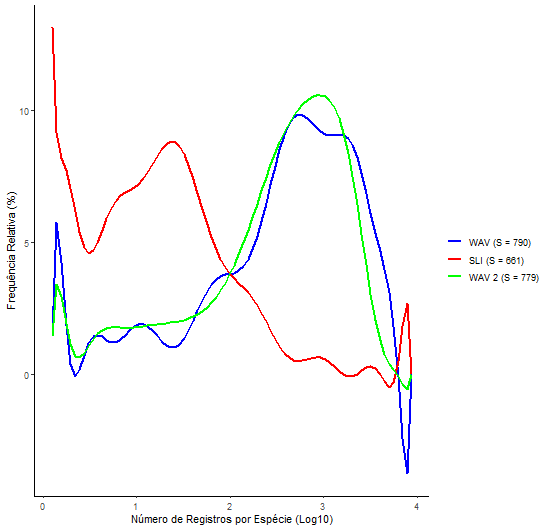
\includegraphics[height = 6cm]{Imagens/133.png}
\\{\scriptsize Figura 3: Distribuição de espécies em classes segundo o número de registros (Log10), em cada banco de dados: WAV = Wikiaves, SLI = SpeciesLink, WAV2 = WAV com municípios redundantes em SLI. S = número de espécies.}
\label{fig03}
\end{figure}

\newpage

\item Altitude

\begin{figure}[h!]
\centering
{\scriptsize Tabela 5: Estatísticas de tendência central e dispersão para a altitude (m) da sede dos municípios em cada banco de dados: WAV = Wikiaves, SLI = SpeciesLink. n = número de municípios, m = média, dp = desvio-padrão, min-max = valores extremos, q1-q3 = quartis. Foram excluídos dessa análise os municípios com altitude inferior a 250 m e superior a 1200 m.}
\\
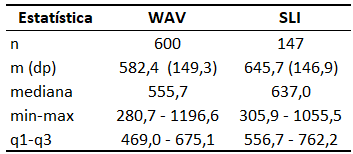
\includegraphics[height = 3cm]{Tabelas/5.png}
\label{t05}
\end{figure}

\begin{figure}[h!]
\centering
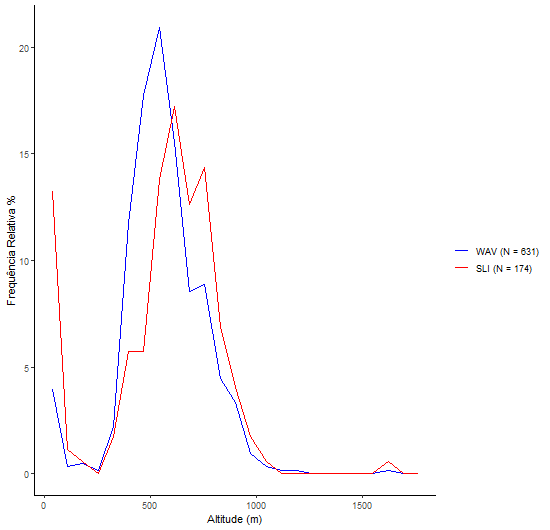
\includegraphics[height = 6cm]{Imagens/213.png}
\\{\scriptsize Figura 4: Distribuição de municípios em classes segundo a altitude (m) de sua sede em cada banco de dados: WAV = Wikiaves, SLI = SpeciesLink. n = número de municípios. Foram excluídos da análise da Tabela 5 os municípios com altitude inferior a 250 m e superior a 1200 m.}
\end{figure}

\item Área

\begin{figure}[h!]
\centering
{\scriptsize Tabela 6: Estatísticas de tendência central e dispersão para a área (Log10 km2) dos municípios em cada banco de dados: WAV = Wikiaves, SLI = SpeciesLink. n = número de municípios, m = média, dp = desvio-padrão, min-max = valores extremos, q1-q3 = quartis. Foram excluídos dessa análise os municípios com área inferior a 20 km2 no WAV e 40km2 no SLI.}
\\
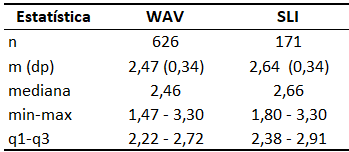
\includegraphics[height = 3cm]{Tabelas/6.png}
\end{figure}

\newpage

\begin{figure}[h!]
\centering
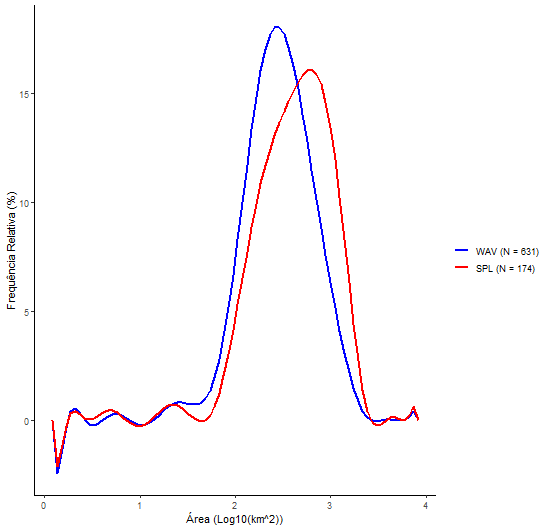
\includegraphics[height = 6cm]{Imagens/223.png}
\\{\scriptsize Figura 5: Distribuição de municípios em classes segundo a área (Log10 km2) em cada banco de dados: WAV = Wikiaves, SLI = SpeciesLink. n = número de municípios. Foram excluídos da análise da Tabela 6 os municípios com área inferior a 20 km2 no WAV e 40km2 no SLI.}
\end{figure}


\item População

\begin{figure}[h!]
\centering
{\scriptsize Tabela 7: Estatísticas de tendência central e dispersão para o tamanho da população humana (Log10 indivíduos) dos municípios em cada banco de dados: WAV = Wikiaves, SLI = SpeciesLink. n = número de municípios, m = média, dp = desvio-padrão, min-max = valores extremos, q1-q3 = quartis. Foi excluído dessa análise o município com 12252023 habitantes (São Paulo).}
\\
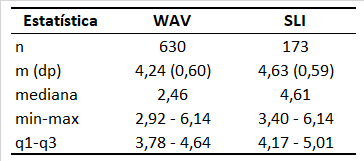
\includegraphics[height = 3cm]{Tabelas/7.png}
\end{figure}



\begin{figure}[h!]
\centering
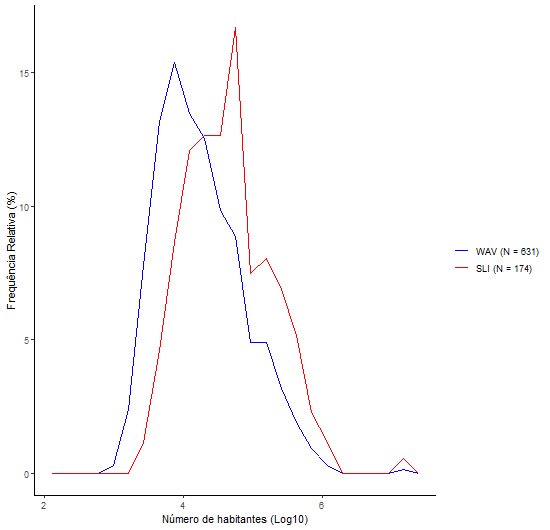
\includegraphics[height = 6cm]{Imagens/233.png}
\\{\scriptsize Figura 6: Distribuição de municípios em classes segundo o tamanho da população humana (Log10 indivíduos) em cada banco de dados: WAV = Wikiaves, SLI = SpeciesLink. n = número de municípios. Foi excluído da análise da Tabela 7 o município com 12252023 habitantes (São Paulo).}
\end{figure}

\newpage

\item Latitude

\begin{figure}[h!]
\centering
{\scriptsize Tabela 8: Estatísticas de tendência central e dispersão para a latitude (graus) da sede dos municípios em cada banco de dados: WAV = Wikiaves, SLI = SpeciesLink. n = número de municípios, m = média, dp = desvio-padrão, min-max = valores extremos, q1-q3 = quartis.}
\\
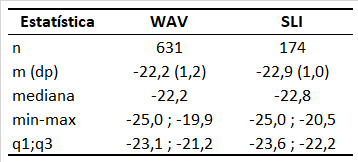
\includegraphics[height = 3cm]{Tabelas/8.png}
\end{figure}



\begin{figure}[h!]
\centering
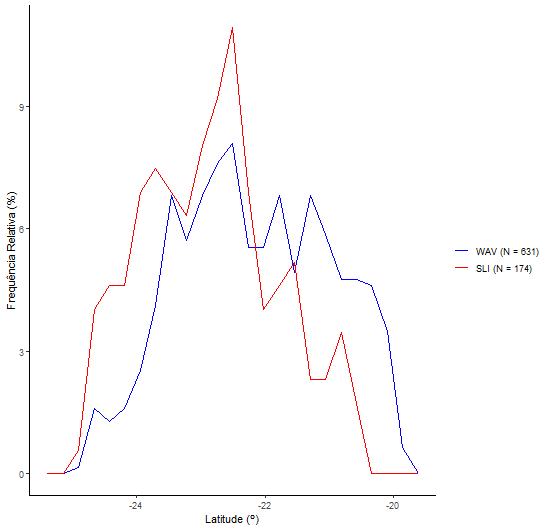
\includegraphics[height = 6cm]{Imagens/243.png}
\\{\scriptsize Figura 7: Distribuição de municípios em classes a latitude (graus) da sede dos municípios em cada banco de dados: WAV = Wikiaves, SLI = SpeciesLink. n = número de municípios.}
\end{figure}

\item Longitude


\begin{figure}[h!]
\centering
{\scriptsize Tabela 9: Estatísticas de tendência central e dispersão para a longitude (graus) da sede dos municípios em cada banco de dados: WAV = Wikiaves, SLI = SpeciesLink. n = número de municípios, m = média, dp = desvio-padrão, min-max = valores extremos, q1-q3 = quartis.}
\\
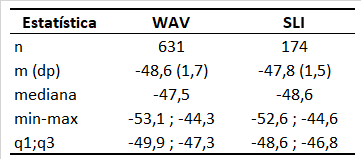
\includegraphics[height = 3cm]{Tabelas/9.png}
\end{figure}


\begin{figure}[h!]
\centering
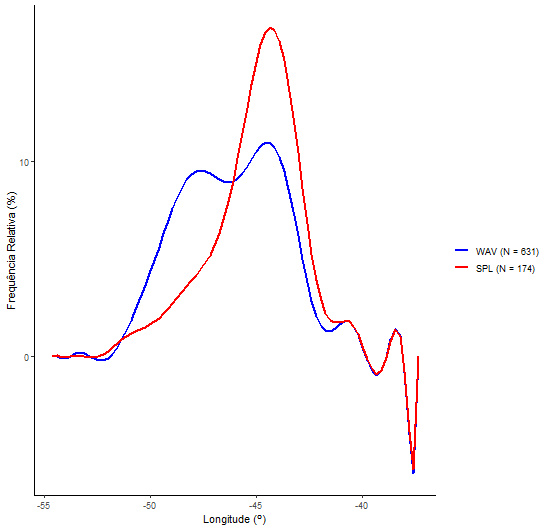
\includegraphics[height = 6cm]{Imagens/253.png}
\\{\scriptsize Figura 8: Distribuição de municípios em classes a longitude (graus) da sede dos municípios em cada banco de dados: WAV = Wikiaves, SLI = SpeciesLink. n = número de municípios.}
\end{figure}

\end{itemize}

\newpage

\subsection{Análise Bivariada}

\begin{itemize}

\item Registros

\begin{figure}[h!]
\centering
{\scriptsize Tabela 10. Correlação linear entre o número de registros (Log10) por município em cada banco de dados e variáveis explanatórias. WAV = Wikiaves, SLI = SpeciesLink, WAV2 = WAV com municípios redundantes em SLI. Número de municípios (n), coeficiente de correlação de Pearson (r) para cada pareamento, com outliers bivariados excluídos. Valores significantes $(p < 0.05)$ em negrito. }
\\
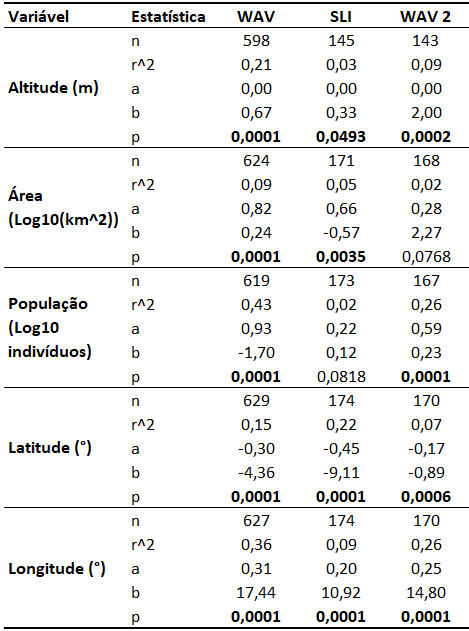
\includegraphics[height = 11cm]{Tabelas/10.png}
\end{figure}

\newpage

\begin{itemize}

\item Altitude

\begin{figure}[h!]
\centering
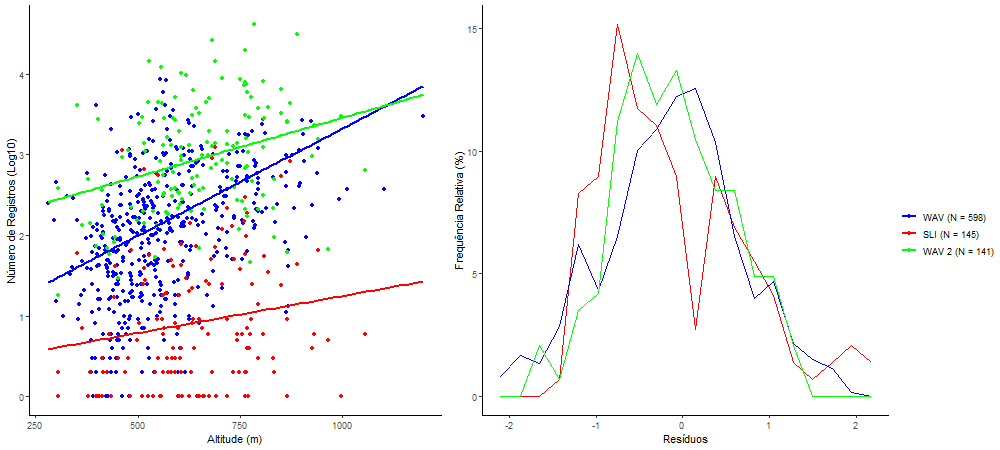
\includegraphics[width = 15cm]{Imagens/31113.png}
\\{\scriptsize Figura 9. Relação linear entre o número de registros (Log10) em cada banco de dados e a altitude (m) da sede dos municípios (esquerda) e respectiva distribuição de resíduos (direita, em unidades de desvio-padrão, em unidades de desvio-padrão). Outliers bivariados foram excluídos. }
\end{figure}


\item Área


\begin{figure}[h!]
\centering
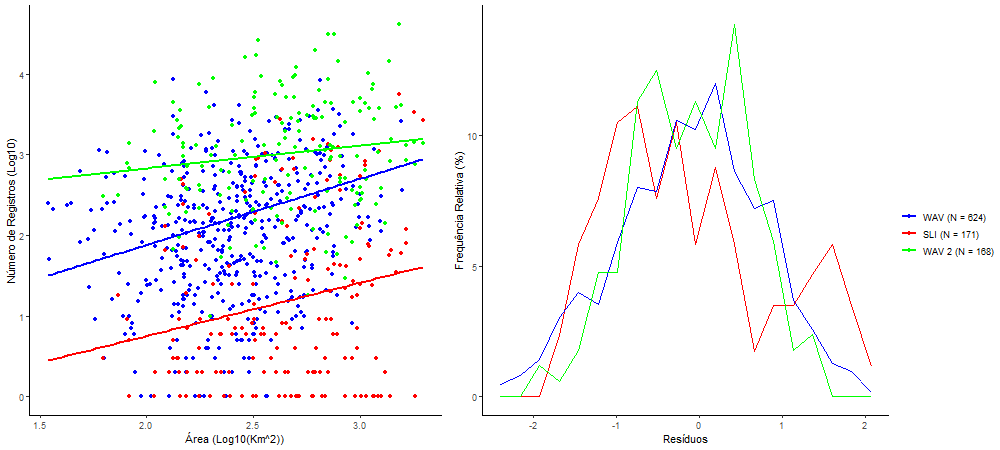
\includegraphics[width = 15cm]{Imagens/31213.png}
\\{\scriptsize Figura 10. Relação linear entre o número de registros (Log10) em cada banco de dados e a área (Log10 km2) dos municípios (esquerda) e respectiva distribuição de resíduos (direita, em unidades de desvio-padrão). Outliers bivariados foram excluídos.}
\end{figure}

\item População

\begin{figure}[h!]
\centering
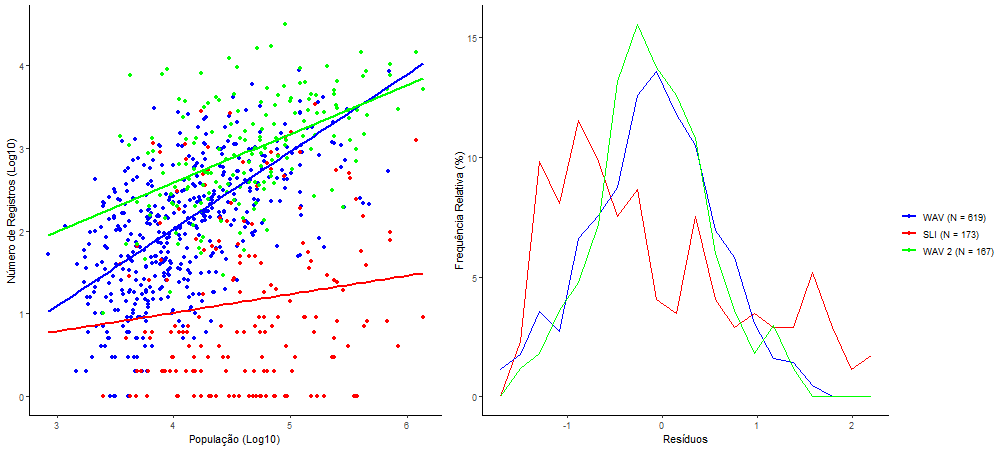
\includegraphics[width = 15cm]{Imagens/31313.png}
\\{\scriptsize Figura 11. Relação linear entre o número de registros (Log10) em cada banco de dados e o tamanho da população humana (Log10 indivíduos) dos municípios (esquerda) e respectiva distribuição de resíduos (direita, em unidades de desvio-padrão). Outliers bivariados foram excluídos.}
\end{figure}

\newpage

\item Latitude

\begin{figure}[h!]
\centering
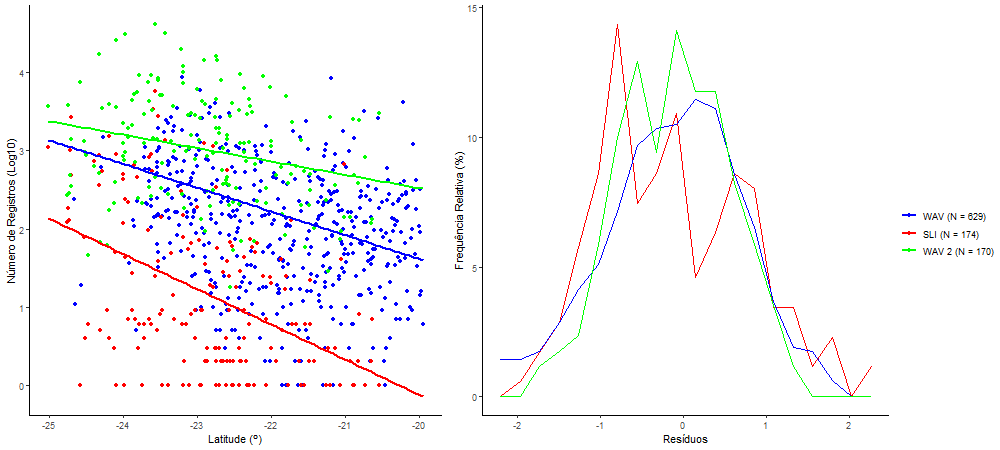
\includegraphics[width = 15cm]{Imagens/31413.png}
\\{\scriptsize Figura 12. Relação linear entre o número de registros (Log10) em cada banco de dados e a latitude (graus) da sede dos municípios (esquerda) e respectiva distribuição de resíduos (direita, em unidades de desvio-padrão). Outliers bivariados foram excluídos.}
\end{figure}

\item Longitude

\begin{figure}[h!]
\centering
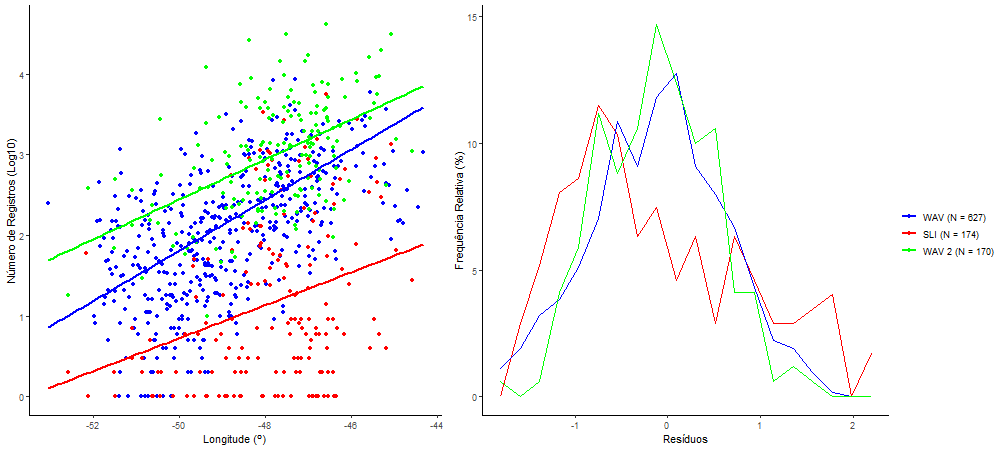
\includegraphics[width = 15cm]{Imagens/31513.png}
\\{\scriptsize Figura 13. Relação linear entre o número de registros (Log10) em cada banco de dados e a longitude (graus) da sede dos municípios (esquerda) e respectiva distribuição de resíduos (direita, em unidades de desvio-padrão). Outliers bivariados foram excluídos.}
\end{figure}

\newpage

\end{itemize}

\item Espécies

\begin{figure}[h!]
\centering
{\scriptsize Tabela 11: Correlação linear entre o número de espécies (Log10) por município em cada banco de dados e variáveis explanatórias. WAV = Wikiaves, SLI = SpeciesLink, WAV2 = WAV com municípios redundantes em SLI. Número de municípios (n), coeficiente de correlação de Pearson (r) para cada pareamento, com outliers bivariados excluídos. Valores significantes $(p < 0.05)$ em negrito.}
\\
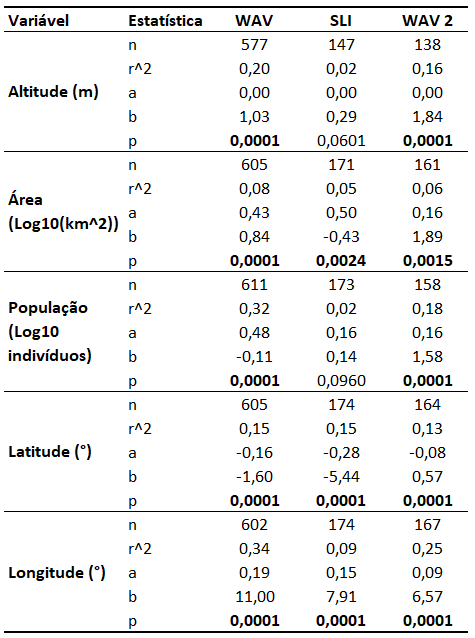
\includegraphics[height = 10cm]{Tabelas/11.png}
\end{figure}

\begin{itemize}


\item Altitude

\begin{figure}[h!]
\centering
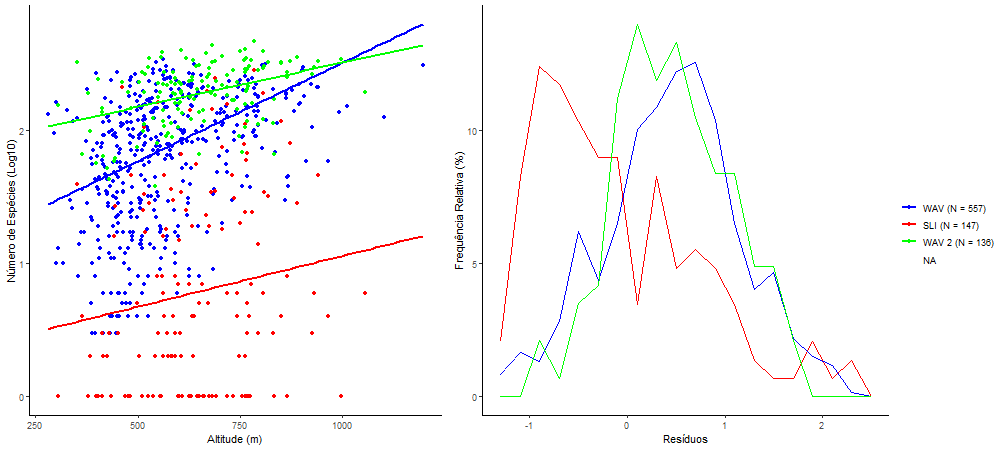
\includegraphics[width = 15cm]{Imagens/32113.png}
\\{\scriptsize Figura 14: Relação linear entre o número de espécies (Log10) em cada banco de dados e a altitude (m) da sede dos municípios (esquerda) e respectiva distribuição de resíduos (direita, em unidades de desvio-padrão). Outliers bivariados foram excluídos.}
\end{figure}



\item Área



\begin{figure}[h!]
\centering
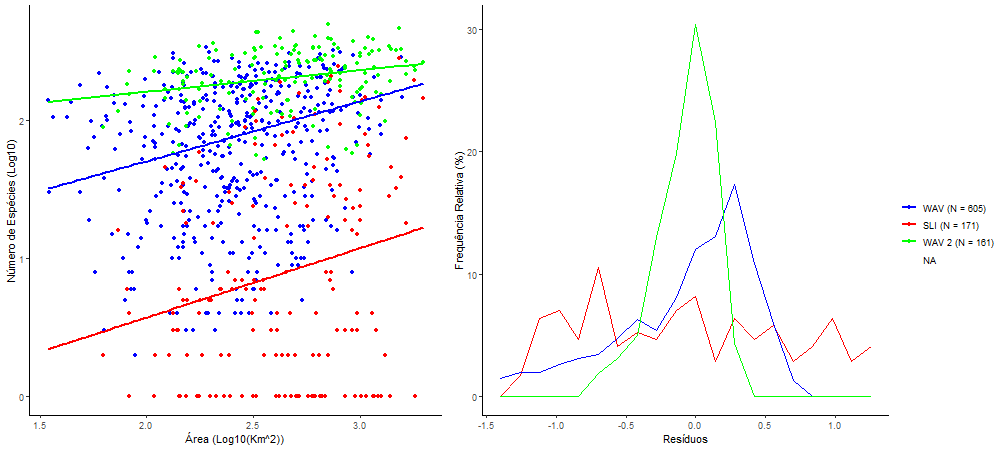
\includegraphics[width = 15cm]{Imagens/32213.png}
\\{\scriptsize Figura 15: Relação linear entre o número de espécies (Log10) em cada banco de dados e a área (Log10 km2) dos municípios (esquerda) e respectiva distribuição de resíduos (direita, em unidades de desvio-padrão). Outliers bivariados foram excluídos.}
\end{figure}

\newpage

\item População

\begin{figure}[h!]
\centering
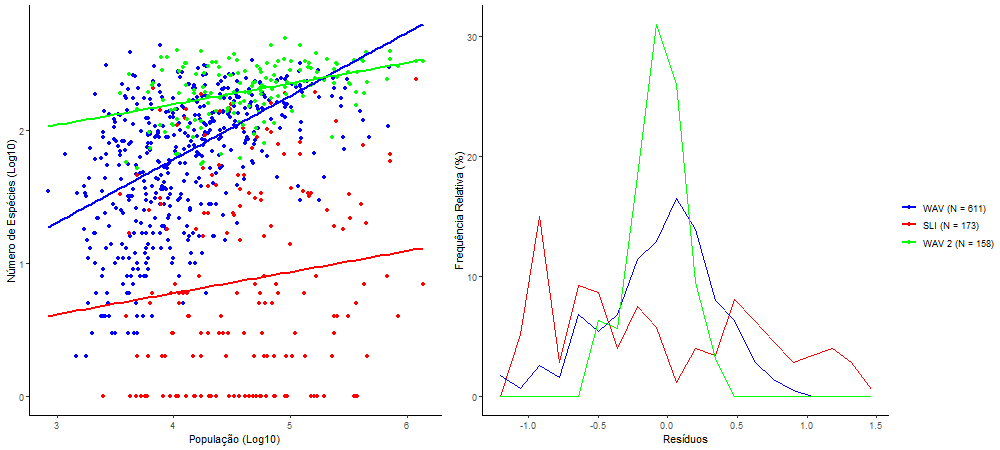
\includegraphics[width = 15cm]{Imagens/32313.png}
\\{\scriptsize Figura 16: Relação linear entre o número de espécies (Log10) em cada banco de dados e o tamanho da população humana (Log10 indivíduos) dos municípios (esquerda) e respectiva distribuição de resíduos (direita, em unidades de desvio-padrão). Outliers bivariados foram excluídos.}
\end{figure}


\item Latitude

 

\begin{figure}[h!]
\centering
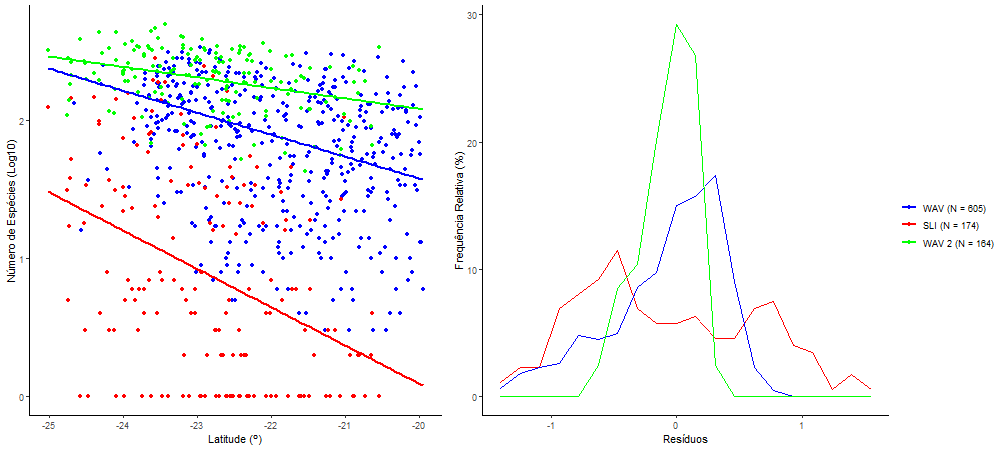
\includegraphics[width = 15cm]{Imagens/32413.png}
\\{\scriptsize Figura 17: Relação linear entre o número de espécies (Log10) em cada banco de dados e a latitude (graus) da sede dos municípios (esquerda) e respectiva distribuição de resíduos (direita, em unidades de desvio-padrão). Outliers bivariados foram excluídos.}
\end{figure}

\newpage

\item Longitude

\begin{figure}[h!]
\centering
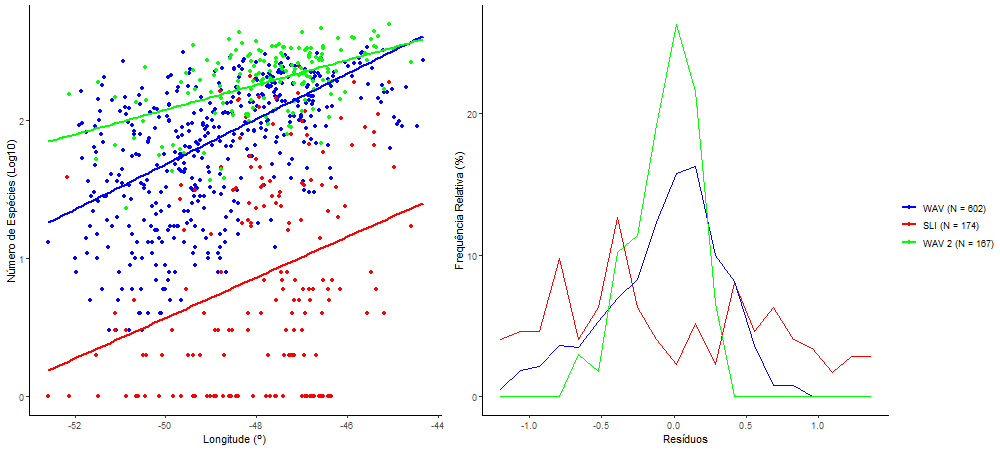
\includegraphics[width = 15cm]{Imagens/32513.png}
\\{\scriptsize Figura 18: Relação linear entre o número de espécies (Log10) em cada banco de dados e a longitude (graus) da sede dos municípios (esquerda) e respectiva distribuição de resíduos (direita, em unidades de desvio-padrão). Outliers bivariados foram excluídos.}
\end{figure}

\end{itemize}

\item Variáveis preditoras 

\begin{itemize}

\item Registros

\begin{figure}[h!]
\centering
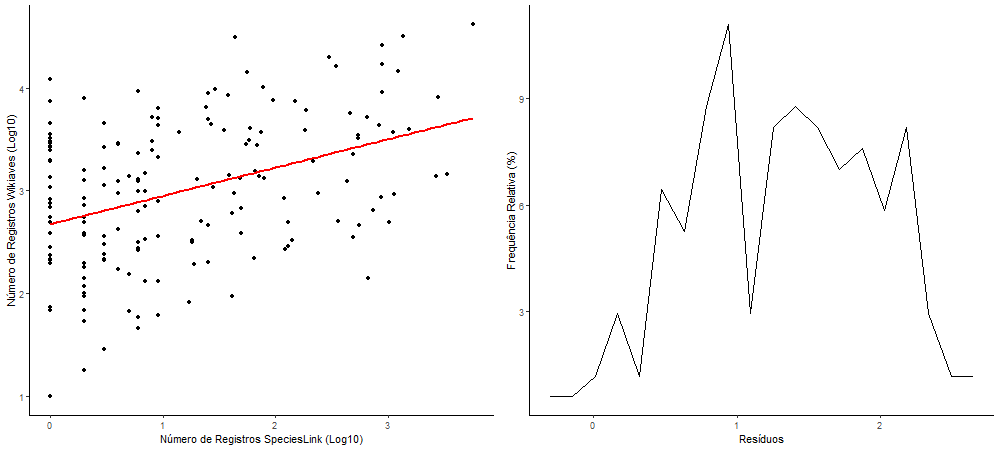
\includegraphics[width = 12cm]{Imagens/4113.png}
\\{\scriptsize  Figura 19: Relação linear entre o número de registros (Log10) nos bancos de dados SLI e WAV2 pareados por X municípios redundantes e respectiva distribuição de resíduos (direita, em unidades de desvio-padrão). Outliers bivariados foram excluídos. n = 171, r2 = 0,1588, P $<$ 0,0001 .}
\end{figure}

\newpage

\item Espécies

\begin{figure}[h!]
\centering
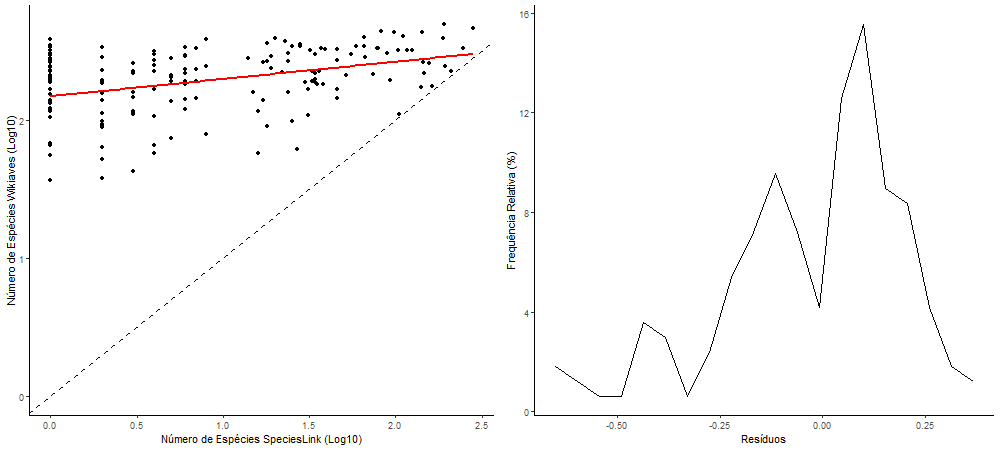
\includegraphics[width = 12cm]{Imagens/4213.png}
\\{\scriptsize Figura 20: Relação linear entre o número de espécies (Log10) nos bancos de dados SLI e WAV2 pareados por X municípios redundantes e respectiva distribuição de resíduos (direita, em unidades de desvio-padrão). Outliers bivariados foram excluídos. n = 167 , r2 = 0,1523 , P $<$ 0,0001 .}
\end{figure}

\item Registros x Espécies

\begin{figure}[h!]
\centering
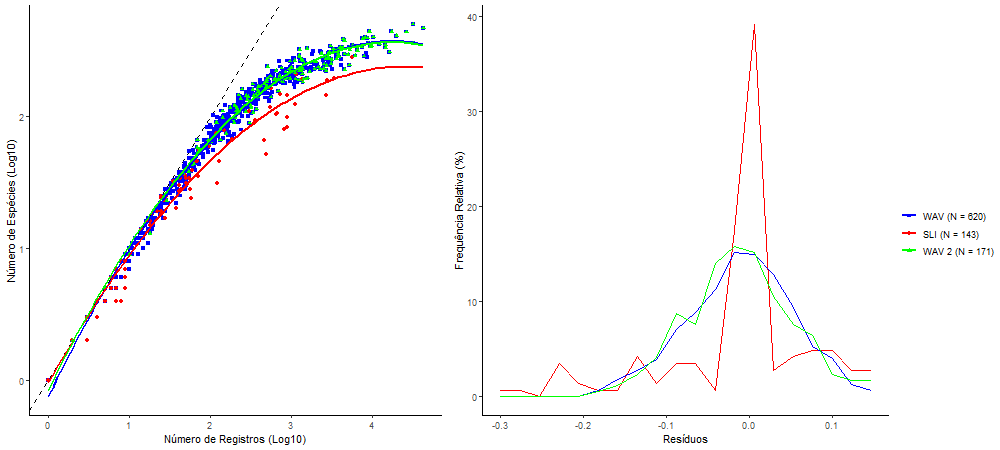
\includegraphics[width = 15cm]{Imagens/4333.png}
\\{\scriptsize Figura 21: Relação quadrática entre o número de espécies e o número de registros (ambos em Log10) nos bancos de dados WAV, SLI e WAV2 pareados por município e respectiva distribuição de resíduos (direita, em unidades de desvio-padrão). Outliers bivariados foram excluídos. n = 620, r2 = 0,9875, P $<$ 0,0001 no Wikiaves. n = 143, r2 = 0,9867, P $<$ 0,0001 no Wikiaves. n = 171, r2 = 0,9647, P $<$ 0,0001 no Wikiaves 2.}
\end{figure}

\end{itemize}

\item Distribuição Geográfica

\begin{figure}[h!]
\centering
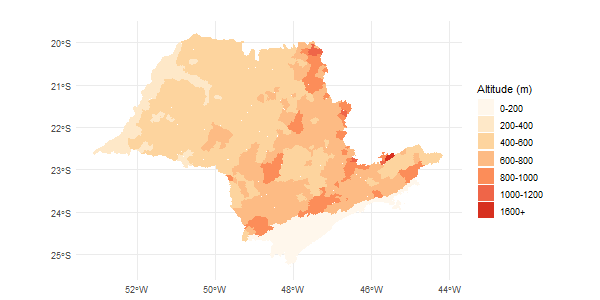
\includegraphics[width = 10cm]{Imagens/511.png}
\\{\scriptsize Figura 22: Distribuição espacial dos municípios do estado de São Paulo em classes segundo a altitude (m) de sua sede.}
\end{figure}

\begin{figure}[h!]
\centering
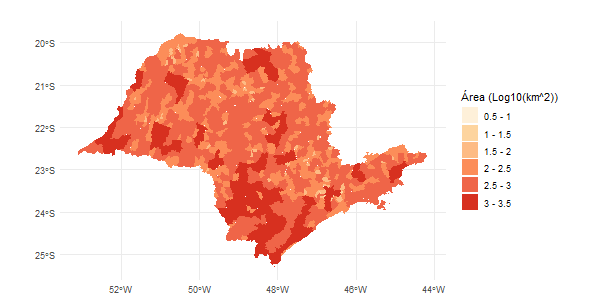
\includegraphics[width = 10cm]{Imagens/521.png}
\\{\scriptsize Figura 23: Distribuição espacial dos municípios do estado de São Paulo em classes segundo a área (Log10 km2).}
\end{figure}

\begin{figure}[h!]
\centering
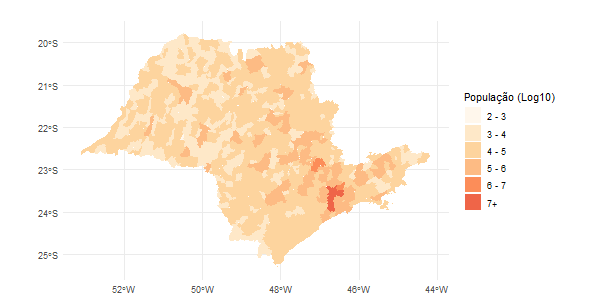
\includegraphics[width = 10cm]{Imagens/531.png}
\\{\scriptsize Figura 24: Distribuição espacial dos municípios do estado de São Paulo em classes segundo o tamanho da população humana (Log10 indivíduos).}
\end{figure}

\begin{figure}[h!]
\centering
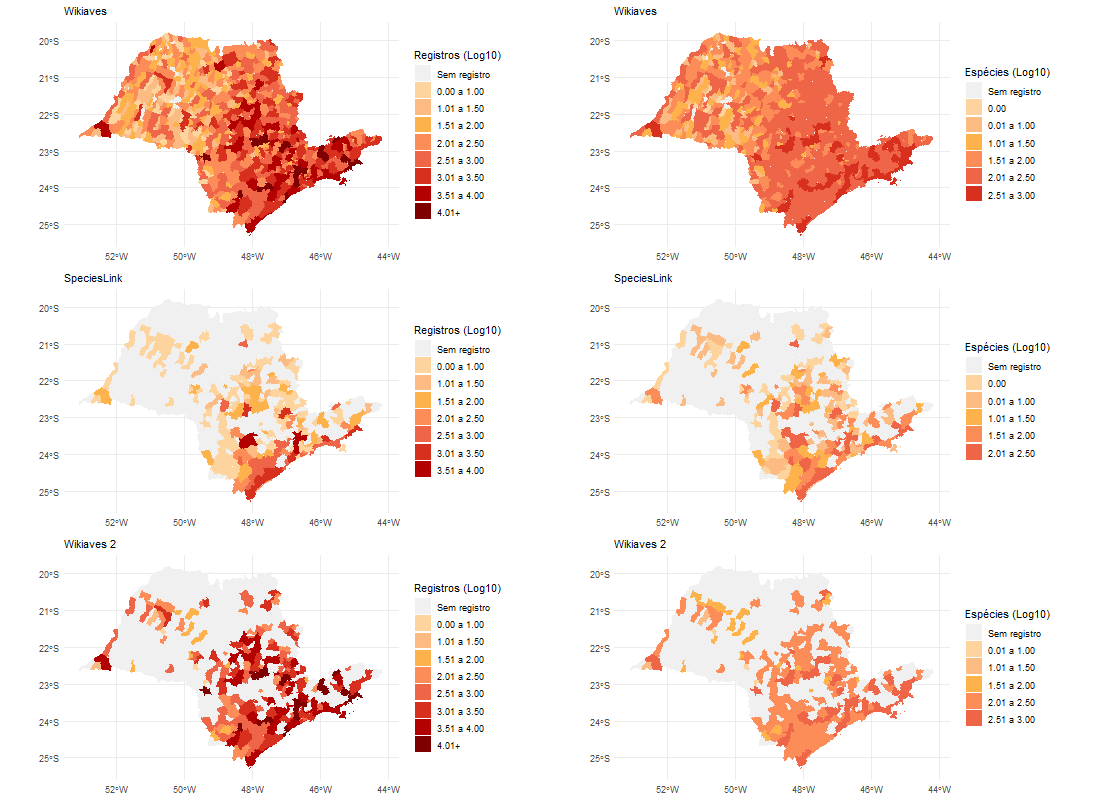
\includegraphics[width = 15cm]{Imagens/561.png}
\\{\scriptsize Figura 25: Distribuição espacial dos municípios do estado de São Paulo em classes segundo o número de registros (Log10, esquerda) e o número de espécies (Log10, direita) em cada banco de dados (WAV = superior, SLI = central, WAV2 = inferior).}
\end{figure}

\end{itemize}

\newpage
